\documentclass{../ossphysics}
\usepackage{circuitikz}

\begin{document}
\setheader{Grade 11 Physics Class 15 Homework}
\hwtitle{11}{15}{Transformers and Power Generation}

\begin{questions}

  % DID NOT DISCUSS THIS IN CLASS
  %\question Which of the following determines the amount of current produced
  %in a conductor by a changing magnetic field?
  %\begin{choices}
  %  \choice the rate of change of the magnetic field
  %  \choice the strength of the magnetic field
  %  \choice coiling the conductor
  %  \choice all of the above
  %\end{choices}

  %\question For a single-loop AC electric generator, the current produced is
  %zero when the plane of the loop is at which angles relative to the magnetic
  %field?
  %\begin{choices}
  %  \choice \ang{0} and \ang{180}
  %  \choice \ang{45} and \ang{135}
  %  \choice \ang{90} and \ang{270}
  %  \choice \ang{90} and \ang{180}
  %\end{choices}

  \question Which of the following correctly describes a step-up transformer?
  \begin{choices}
    \choice The number of windings on the primary coil is greater than the
    number of windings on the secondary coil.
    \choice The current in the primary coil is less than the current in the
    secondary coil.
    \choice The voltage on the primary coil is less than the voltage on the
    secondary coil.
    \choice The ratio of primary windings to the number of secondary windings
    is greater than one.
  \end{choices}

  \question Which of the following does not change in an ordinary transformer?
  \begin{choices}
    \choice Frequency
    \choice Voltage
    \choice Current
    \choice All of the above
    \choice None of the above
  \end{choices}
  
  \question Which of the following descriptions would provide the most efficient
  electrical energy transmission?
  \begin{choices}
    \choice low-voltage and high-current DC
    \choice high-voltage and low-current AC
    \choice low-voltage and high-current AC
    \choice high-voltage and high-current AC
  \end{choices}

  \question Which winding in a transformer has more number of turns?
  \begin{choices}
    \choice Low voltage winding
    \choice Primary winding
    \choice High voltage winding
    \choice Secondary winding
  \end{choices}

  \question The primary and secondary windings of a transformer are
  \underline{\hspace{1in}}
  \begin{choices}
    \choice electrically coupled 
    \choice magnetically coupled
    \choice capacitively coupled 
    \choice physically coupled
  \end{choices}
  
  \question A transformer is used to reduce the mains supply of
  \SI{220}{\volt} to \SI{22}\volt. If the currents in the primary and
  secondary are \SI2{\ampere} and \SI{15}{\ampere} respectively, what is the
  efficiency of the transformer?
  \begin{choices}
    \choice\SI{65}\percent
    \choice\SI{75}\percent
    \choice\SI{80}\percent
    \choice\SI{90}\percent
  \end{choices}
  \newpage
  
  \question Do electrons travel from the power plant to your home to provide
  electrical energy? Explain your answer.
  \vspace{1.5in}
  
  %\question In alternating current electricity, is the voltage proportional
  %to the current? Explain.

  %\question In the figure below, a small coil falls downwards into a larger
  %coil and a current is directed through the large coil in the direction shown.
  %
  %\begin{minipage}{.35\textwidth}
  %  \pic1{graphics/stacked-coils}
  %\end{minipage}
  %\begin{minipage}{.6\textwidth}
  %  \begin{parts}
  %    \part What is the direction of the magnetic field induced by the current
  %    inside the larger coil?
  %    \part What is the direction of the current in the small coil induced by
  %    the magnetic field of the small coil? (The current in the small coil
  %    would generate a magnetic field that opposes the magnetic field from the
  %    larger coil.)
  %    %\part What is the direction of the magnetic field induced by the current
  %    %in the large coil?
  %    %\part What is the direction of the magnetic field induced by the small
  %    %coil?
  %  \end{parts}
  %\end{minipage}

  \question Calculate the current through, and voltage across the load in this
  transformer circuit: 
  \begin{center}
    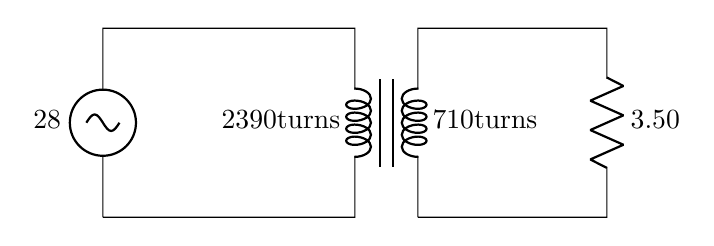
\begin{tikzpicture}[scale=.8]
      \draw (0,0) to[sinusoidal voltage source,l=\SI{28}\volt] (0,3)--(4,3)
      to[inductor,l_=\SI{2390}{turns}] (4,0)--(0,0);
      \draw (5,0) to[inductor,l_=\SI{710}{turns}] (5,3)--(8,3)
      to[R,l=\SI{3.50}{\ohm}] (8,0)--(5,0);
      \draw[thick] (4.4,.8)--(4.4,2.2);
      \draw[thick] (4.6,.8)--(4.6,2.2);
    \end{tikzpicture}
  \end{center}
  \vspace{\stretch{.8}}

  \question A transformer has 500 turns of the primary winding and 10 turns of
  the secondary winding.
  \begin{parts}
    \part Determine the secondary voltage if the secondary circuit is open and
    the primary voltage is \SI{120}\volt.

    \part Determine the current in the primary and secondary winding, given
    that the secondary winding is connected to a resistance load \SI{15}\ohm?
  \end{parts}
  \vspace{\stretch1}
  \newpage
  
  \fullwidth{
    \centering
    \textbf{REVIEW QUESTIONS}
  }
  
  \question A Sky Screamer Extreme water slide at the West Edmonton Mall has a
  height of \SI{26}\metre. If a \SI{45}{\kilo\gram} child begins at the top of
  the slide with a speed of \SI{.50}{\metre\per\second},
  \begin{parts}
    \part What is her speed at the bottom of the slide, if friction can be
    neglected?
    \part If she only reaches a speed of \SI{60}{\kilo\metre\per\hour}, what
    fraction of energy was lost?
    \part After the child exits the water slide, the force exerted on her by the
    pool slows her to a stop in a distance of \SI{6.0}\metre. What is the work
    done by the the water? 
  \end{parts}
  \vspace{\stretch1}
  
  \question A \SI{250}{mL} cup of water is too hot to drink at \SI{85}\celsius,
  so it is poured into a \SI{415}{\gram} ceramic mug container at
  room temperature (\SI{20}\celsius). The mug contained \SI{50}{\gram} of ice at
  \SI{-10}{\celsius} when the water is poured. What is the final temperature of 
  the water? Assume that all the ice has melted, and that no heat is lost to the
  surroundings. The specific heat capacities of the ceramic cup, water, and ice
  are $c_\text{cup}=\SI{1085}{\joule\per\kilo\gram.\celsius}$,
  $c_\text{ice}=\SI{2090}{\joule\per\kilo\gram.\celsius}$, and
  $c_\text{water}=\SI{4186}{\joule\per\kilo\gram.\celsius}$ respectively. The
  density of water is $\rho=\SI{1000}{\kilo\gram\per\metre\cubed}$. (Conversion
  factor: $\SI1{\metre\cubed}=\SI{1000}L$)
  \vspace{\stretch1}

%  \question In class we used two different equations for the speed of sound.
%  Calculate the percentage error between the equations at a temperature of
%  \SI{45}\celsius.
  
%  \question A wind power plant produces \SI{12}{\mega\watt} of power that is
%  stepped up to a potential difference of \SI{1.00e2}{\kilo\volt} for
%  transmission. If there is a \SI{.90}{\percent} loss of power due to
%  transmission, what is the total resistance in the transmission wire? Assume
%  there is no power loss in the transformer.

%  \question A power plant produces 1800 MW of power at a current of
%  \SI{30.}{\kilo\ampere}. The power is then stepped up to a voltage of
%  \SI{240}{\kilo\volt}. If the primary circuit used in the transformer has
%  100 windings, how many windings are used in the secondary circuit? Assume
%  there is no power loss in the transformer.
  
  %\question A modified transformer in the figure below has a normal primary
  %circuit, but two secondary circuits. The same winding-to-voltage ratio holds
  %for each segment.
  %
  %\begin{minipage}{.35\textwidth}
  %  \pic{1}{graphics/transformer1}
  %\end{minipage}
  %\begin{minipage}{.6\textwidth}
  %  \begin{parts}
  %    \part State the equations comparing the primary voltage to the output
  %    voltage for each of the coil segments.
  %    \part Energy must be conserved. Knowing this, write an equation for the
  %    input power compared to the output power and use it to find an equation
  %    relating the input current and voltage to the output currents and
  %    voltages.
  %    \part If $V_p=\SI{120}\volt$, $I_p=\SI{5.}\ampere$, $N_p=100$, $N_1=5$,
  %    and $N_2=20$, what are the two secondary voltages $V_1$ and $V_2$?
  %    \part Why is this type of transformer useful?
  %  \end{parts}
  %\end{minipage}
  
  %\question The primary circuit of a transformer has a potential difference
  %(voltage) of \SI{2.}{\kilo\volt} and a total resistance of \SI{5.00e2}\ohm.
  %The secondary circuit has a potential difference of \SI{1.00e2}{\volt} and 50
  %turns.
  %\begin{parts}
  %  \part How many turns are in the primary coil?
  %  \part What is the resistance in the secondary circuit?
  %\end{parts}
  
  %\question Two coils, $A$ and $B$, are placed in the same magnetic field. Coil
  %$A$ has twice as many coils as $B$, but the material used in coil $B$ has
  %half the resistance of the material used to make coil $A$. The number of
  %loops in a coil is directly proportional to the magnitude of the electric
  %current induced. Knowing this, determine which coil would have more current
  %if the magnetic field were to suddenly drop to zero.
\end{questions}
\end{document}
